\documentclass[a4paper, 11pt]{beamer}
\usepackage[utf8]{inputenc}
\usepackage[T1]{fontenc}
\usepackage[english]{babel}
\usepackage{graphicx}

\usetheme{Warsaw}

\title{KAMISADO}
\author{Valentin BENOZILLO, Mathieu VIOLA, Rémi VIOLA}
\date{\today}

\begin{document}

\begin{frame}
 \titlepage
\end{frame}

\begin{frame}
 \tableofcontents
\end{frame}

\begin{frame}
 \frametitle{Kamisado}
 \begin{center}
  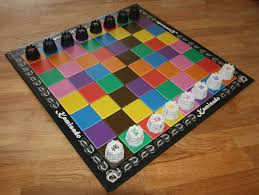
\includegraphics[scale = 0.07]{kamisado.jpeg}
 \end{center}
\end{frame}

\section{The game}
\begin{frame}
 \frametitle{Kamisado}
 \begin{center}
  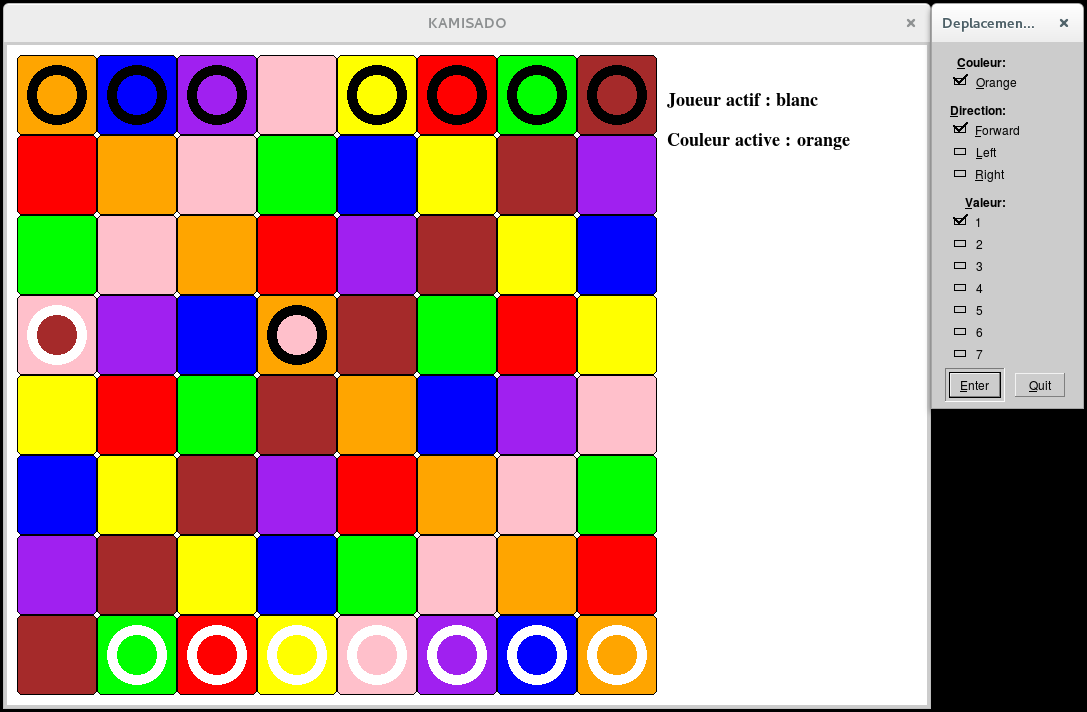
\includegraphics[scale = 0.25]{kamisado.png}
 \end{center}
\end{frame}

\section{The division of the work}
\begin{frame}
 \frametitle{The division of the work}
 \begin{itemize}
  \item Basics of the game by Rémi (k.pl)
  \item Graphical user interface by Rémi (k.pl)
  \item Artificial intelligences by all of us (ia\_firstname.pl)
 \end{itemize}
\end{frame}

\section{The heuristics}
\subsection{Heuristic remi}
\begin{frame}
 \frametitle{The heuristics}
 \framesubtitle{Heuristic remi}
 \begin{table}[htbp]
  \centering
  \begin{tabular}{c c}
    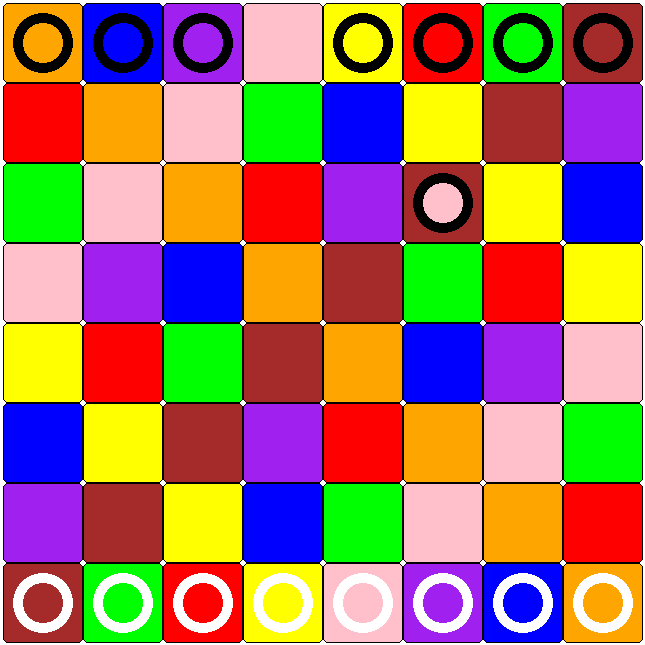
\includegraphics[scale = 0.12]{remi1b.png} & 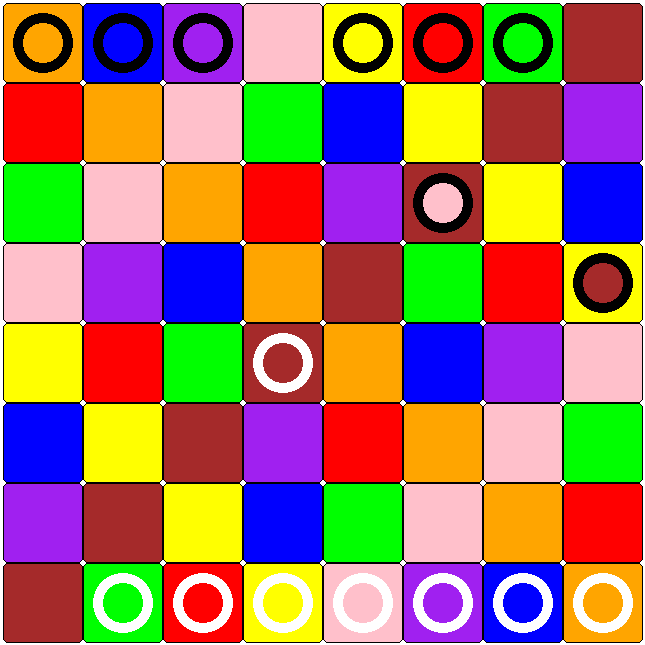
\includegraphics[scale = 0.12]{remi2b.png} \\
    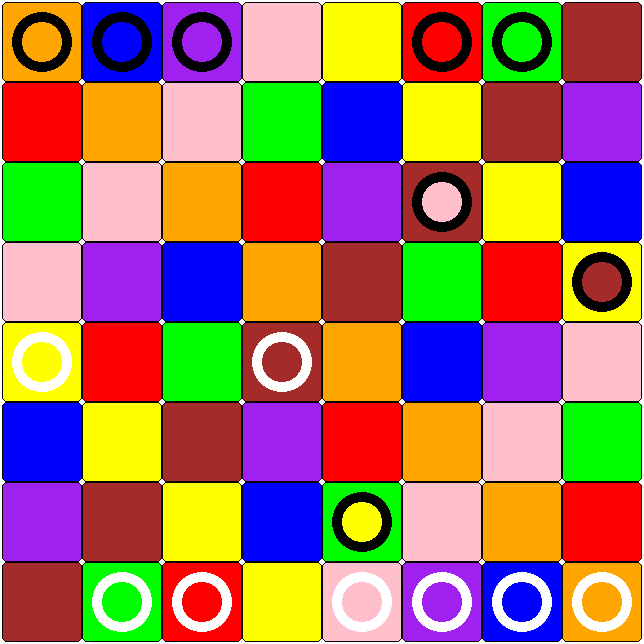
\includegraphics[scale = 0.12]{remi3b.png} & 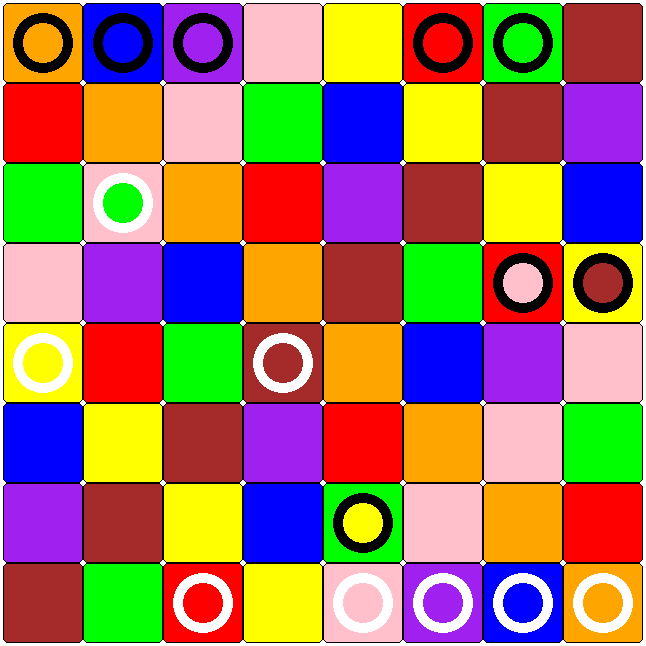
\includegraphics[scale = 0.12]{remi4b.png} \\
  \end{tabular}
  \caption{Four first rounds of a game where AI starts}
 \end{table}
\end{frame}

\subsection{Heuristic valentin}
\begin{frame}
 \frametitle{The heuristics}
 \framesubtitle{Heuristic valentin}
 
\end{frame}

\subsection{Heuristic mathieu}
\begin{frame}
 \frametitle{The heuristics}
 \framesubtitle{Heuristic mathieu}
 
\end{frame}

\subsection{Heuristic mathieu2}
\begin{frame}
 \frametitle{The heuristics}
 \framesubtitle{Heuristic mathieu2}
 
\end{frame}

\subsection{Heuristic mathieu3}
\begin{frame}
 \frametitle{The heuristics}
 \framesubtitle{Heuristic mathieu}
 
\end{frame}

\subsection{Heuristic mathieu4}
\begin{frame}
 \frametitle{The heuristics}
 \framesubtitle{Heuristic mathieu}
 
\end{frame}

\section{The balance sheet}
\subsection{Negative points}
\begin{frame}
 \frametitle{The balance sheet}
 \framesubtitle{Negative points}
 \begin{itemize}
  \item Graphical user interface : Not rather intuitive and ergonomic
  \item 
  \item 
 \end{itemize}
\end{frame}

\subsection{Positive points}
\begin{frame}
 \frametitle{The balance sheet}
 \framesubtitle{Positive points}
 \begin{itemize}
  \item 
  \item 
  \item 
 \end{itemize}
\end{frame}

\end{document}
